\documentclass[../main.tex]{subfiles}

\begin{document}

\subsection{The Threat Model}
\subfile{sections/threat-model.tex}

\subsection{System Design}%TODO: this title is a wip
SSL/TLS supports a wide array of ciphers, but they can be roughly
split into two categories: ciphers that support forward secrecy, and
ciphers that do not. Ciphers that offer forward secrecy are ones
wherein a compromised long-term private key does not allow an
adversary to compromise previously eavesdropped, stored
sessions. SSL/TLS's session establishment mechanism is different based
on the category to which the cipher belongs. Consequentially,
depending on the type of cipher used for a given session, our system
must adapt to two, different,control flows. In this section we present
the following: a high level design that is cipher agnostic, a design
that supports ciphers that \textbf{do not} support forward secrecy,
and a design specific to ciphers that \textbf{do} support forward
secrecy.

\subsubsection*{High level design}
% TODO: WIP
In general, regardless of the cipher used, SSL/TLS utilises the
long-term private key to negotiate ephemeral keys for use in the
current session; hence, to secure the long-term private key, we need
to examine the session establishment mechanism. Roughly, SSL/TLS's
handshake can be split into four steps:

\begin{enumerate}
  \item \textbf{Contacting the server, and establishing parameters for
    the session}. Specifically, the exchange of hello messages that
    include: the server's certificate(s) a list of ciphers supported by
    each side (to determine which cipher is to be used for this session),
    \srandom, and \crandom. The random variables are used to derive the
    secret, used to secure communications.
  \item \textbf{Asymmetric key exchange}: based on the cipher
    selected, the client and server determine the asymmetric keys that are
    to be used to exchange the symmetric keys for the session. This step
    is necessary in two scenarios:
    \begin{enumerate}
      \item The client and server both possess public key
        certificates, and both entities wish to verify each other's identity
        during the handshake. We do not consider this case due to its
        rarity. Generally, the client verifies the server as part of the
        SSL/TLS handshake, and the server verifies the identity of the client
        via some other means, such as a username \& password.
      \item The client and server selected a cipher that offers
        forward secrecy. These ciphers function by first exchanging an
        ephemeral asymmetric secret. This secret is then used in negotiating
        the symmetric secret.
    \end{enumerate} In all other cases, the server's asymmetric keys
    are used to negotiate the ephemeral symmetric secret.
  \item \textbf{Ephemeral symmetric key negotiation}: The client and
    server establish the symmetric secret that is used for the current
    session. Calculating the symmetric secret requires the random values
    exchanged in step 1.
  \item \textbf{Verifying the integrity of the just-negotiated keys,
    completing the session establishment}: Both the server and the client
    compute a MAC across the packets exchanged in establishing the
    session. The resultant finished message is encrypted using the
    just-negotiated keys. If both sides successfully verify the MAC, the
    handshake is complete and the session is established. If either side
    fails to verify the MAC, the session is terminated.
\end{enumerate} Figure~\ref{fig:abshandshake} illustrates this
generalized SSL/TLS handshake.

\begin{figure}[H] \centering
  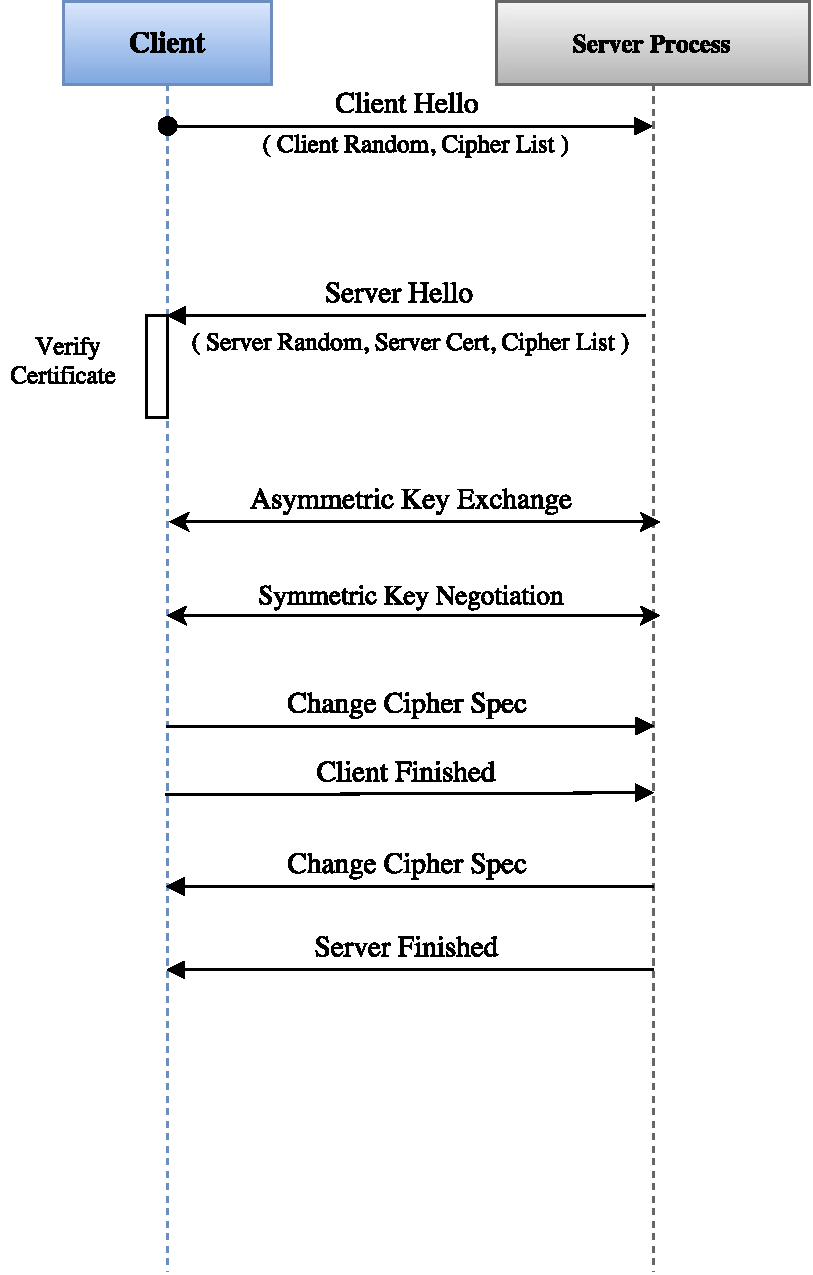
\includegraphics[scale=0.44]{images/abstract-handshake.pdf}
  \caption{SSL/TLS handshake generalization}
  \label{fig:abshandshake}
\end{figure}

By utilizing the aforementioned remote-attestation process, we can
provision the trusted component of the remote server application with
an SSL private key while making it extremely difficult for even
\textit{privileged} processes running on the cloud provider to access
the key. This is a stark contrast to current schemes wherein the
private key is merely shipped as part of the server application to the
cloud provider.

As previously highlighted in Section~\ref{sec:ssloverview}, the
private key is required by a subset of the operations executed during
the handshake step. These operations have to be executed within the
trusted component, and are invoked by the non-trusted component via an
interface that we define in this section. Note that the interface has
to be carefully designed, allowing the handshake to complete correctly
while not exposing the long term private key through an oracle.


% TODO: introduce this better to make it clear that there are 2
% different handshakes; I only went into some detail here, definitely
% need more depth

Take for example an interface where the non-trusted component supplies
\texttt{(ServerRandom, ClientRandom, \{PremasterSecret\}$_K$)}. Such
an interface, while maintaining the secrecy of the private key's bits,
would allow an adversary capable of exploiting the non-trusted
component to generate the symmetric keys for previously eavesdropped
sessions. Therefore, it is no better than leaving the private key in
the non-trusted component.  However, observe that it is not necessary
for \texttt{ServerRandom} to be provided by the non-trusted component,
it need only be provided by the \textit{server}.

% TODO: Cite wedge here somewhere, I do not like how I did it

We can adjust the interface so that the non-trusted component supplies
\texttt{ClientRandom} and \texttt{\{PremasterSecret\}$_k$}, both of
which are generated by the client, and the trusted component generates
a new \texttt{ServerRandom} every time the interface is invoked. The
resulting interface ensures that, even if a previously eavesdropped
\texttt{\{PremasterSecret\}$_K$} is provided, a fresh session-key is
computed on every invocation.

% Freshness of the generated session-key has been used in [WEDGE
% CITATION] to maintain the secrecy of an SSL/TLS private key in the
% face of a passive eavesdropper how can exploit the server
% application's network facing process. We use it to secure the
% private key against an adversary who can exploit the underlying
% operating system and / or a malicious cloud provider.

\subfile{sections/ecdhe-handshake.tex}

\noindent
\\We consider two scenarios that slightly change the exchange of
messages with the enclave during the handshake:
\begin{itemize}
  \item Session keys available to the OS
  \item Session keys hidden inside the enclave and accessible through
    encrypt/decrypt oracle
\end{itemize}

\subfile{latex-images/rsa-handshake.tex}

\paragraph{Session keys available to the OS}

If our sole goal is to protect the long term, private key then we may
decide it is safe to keep the active sessions' keys outside of the
TCB. This allows the compromised OS to use the keys as it pleases. It
can just read them out from memory and send to a man in the middle (on
a different to compromised machine). MITM could then decrypt
previously captured traffic. This method it is possible to leak
current (and cached) sessions keys. Old, captured sessions for which
session keys have been deleted can no longer be recovered. However, if
the OS persists to be malicious it can always monitor future (current)
connections.\\

\noindent
One could prefer this option for performance reasons - such design
puts less burden on the enclave program. In particular the role of the
enclave can finish after the master secret is computed from server and
client randoms and pre-master secret. This is because a pseudo-random
function (PRF) lies between master secret and the input values so no
information can be learned about the private key. The derivation of
session keys and encryption / decryption of messages can be left
unaltered in the untrusted program and therefore less \'context\'
switches to the enclave would be required.

\paragraph{Session keys hidden within the enclave}

One may want to further protect the key material by requiring that the
session keys themselves do not leave the enclave. Instead an encrypt /
decrypt oracle interface is presented to the untrusted component. The
enclave performs the cryptographic operations using stored state
accessed by the session\_id. This prevents the compromised OS from
leaking the session keys to a different machine, but requires a more
complicated and expensive design. One can imagine that if the attacker
is leaking ton of data out of the server, it may be more easily
noticeable than if the session keys are exported outside of the server
once.\\

\noindent
If we decide to keep our session keys in the enclave apart from
providing a mechanism to transfer the cipher context we have to
additionally present an interface that would allow to sign the
handshake finish messages.\\

\noindent
To allow the trusted component to encrypt / decrypt messages we also
need to transfer the symmetric cipher context which can be done during
computation of master secret. Additionally, every time we need to pass
the initialization values such as initialization vector or nonce need
to be transferred to the enclave.\\

\noindent
The performance cost is increased since now at least 4 context
switches between untrusted and trusted processes are required for each
packet processing, i.e. 2 switches to decrypt an incoming packet and
pass plain-text back to the application and 2 to encrypt the outgoing
result after application processing (plain-text in, cipher-text out of
an enclave).\\

\noindent
Also every handshake now needs 6 (TODO: ???) more context switches
during digest update.

\subfile{latex-images/session-keys-inside.tex}

\end{document}
